\section{Data Description and Additional Background}

This appendix collects the material that would have made the main text slower to read. It contains the background and diagnostics that support the empirical setup, allowing the main body to remain focused on the argument and its interpretation.

\subsection{The descriptive role of the asset universe}

The assets were not selected for this dissertation at random. Each instrument represents a distinct part of the traditional financial system, which makes it possible to compare these different parts directly with Bitcoin. Bitcoin is the main object of comparison and is included in every asset pair.

\begin{itemize}
    \item The S\&P~500 is used as a broad measure of U.S. equity-market risk and general investor sentiment.
    \item The NASDAQ Composite represents a more growth-oriented and technology-heavy part of the market, which makes it particularly relevant when studying crypto assets.
    \item Gold and silver ETFs represent exposure to precious metals, a market area often linked to hedging, inflation expectations, and safe-haven discussions.
    \item The U.S. Dollar Index proxy represents defensive positioning and changes in the strength of the U.S. dollar in global markets.
    \item Ethereum is included as a crypto-native comparison asset, allowing same-ecosystem dependence to be compared with dependence across different markets.
\end{itemize}

These assets differ in terms of their investor base, liquidity, sensitivity to broader economic conditions, and importance within the financial system. This variety helps reduce the risk that the conclusions are driven by only one narrow part of the market.

\subsection{Visual overview of the dataset}

Figure~\ref{fig:eda_prices_appendix} shows the normalised price paths for the asset universe. Normalisation sets all series to the same starting point, making differences in the underlying market paths easier to see.

\begin{figure}[H]
    \centering
    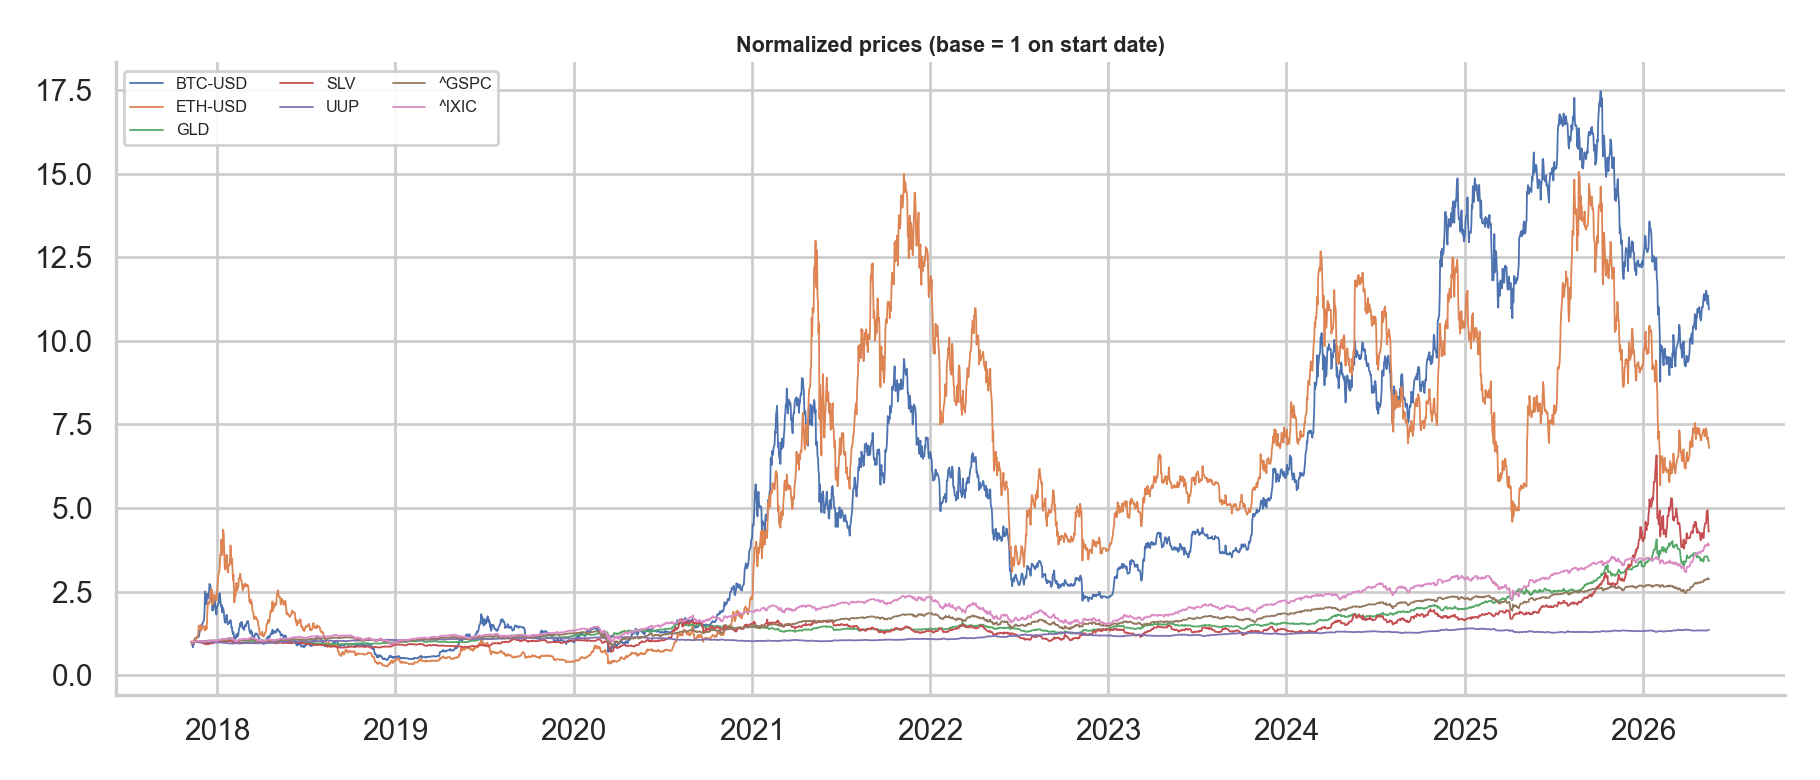
\includegraphics[width=0.95\textwidth]{../outputs/figures/eda_normalized_prices.png}
    \caption{Normalised prices of the assets included in the study.}
    \label{fig:eda_prices_appendix}
\end{figure}

Figure~\ref{fig:eda_vol_appendix} shows the rolling volatility profiles. The profiles show that Bitcoin and the other crypto assets operate in a considerably more volatile environment than the traditional assets. This is another reason for examining dependence as a time-varying process.

\begin{figure}[H]
    \centering
    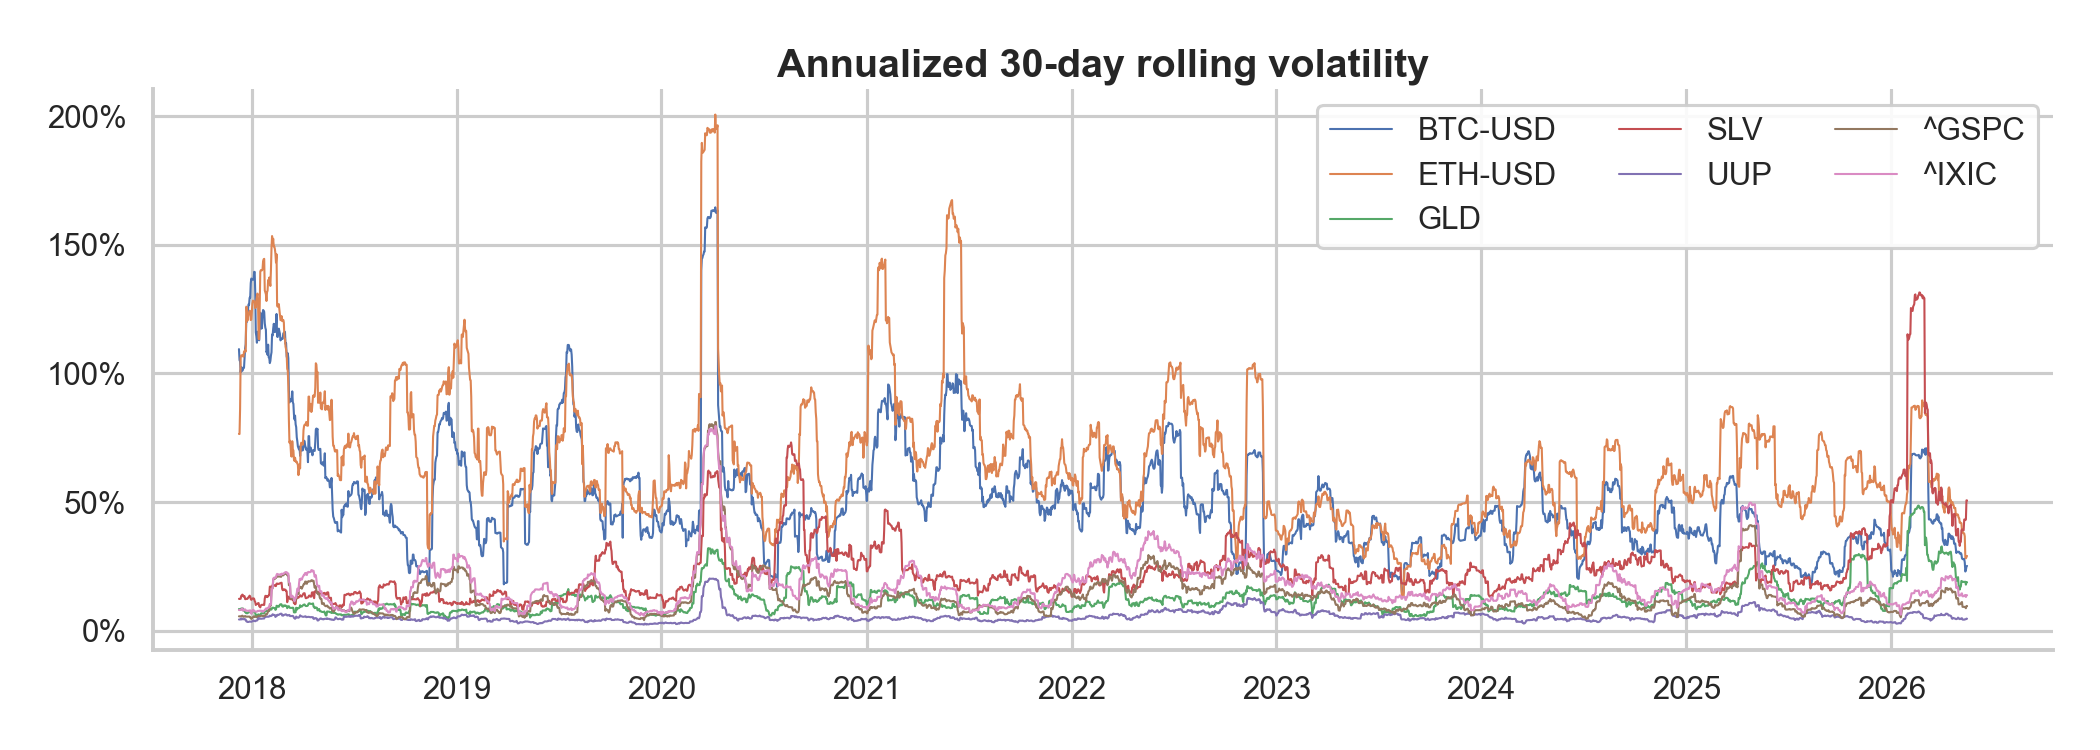
\includegraphics[width=0.95\textwidth]{../outputs/figures/eda_rolling_vol.png}
    \caption{Rolling volatility across the asset universe.}
    \label{fig:eda_vol_appendix}
\end{figure}

Figure~\ref{fig:eda_heatmap_appendix} provides the static correlation heatmap, while the dynamic rolling-correlation structure is shown in the methodology chapter (Figure~\ref{fig:rolling_corr_all}). Taken together, the two figures support the main modelling choice of the thesis: static correlation measures are not sufficient to describe the cross-market relationships studied here.

\begin{figure}[H]
    \centering
    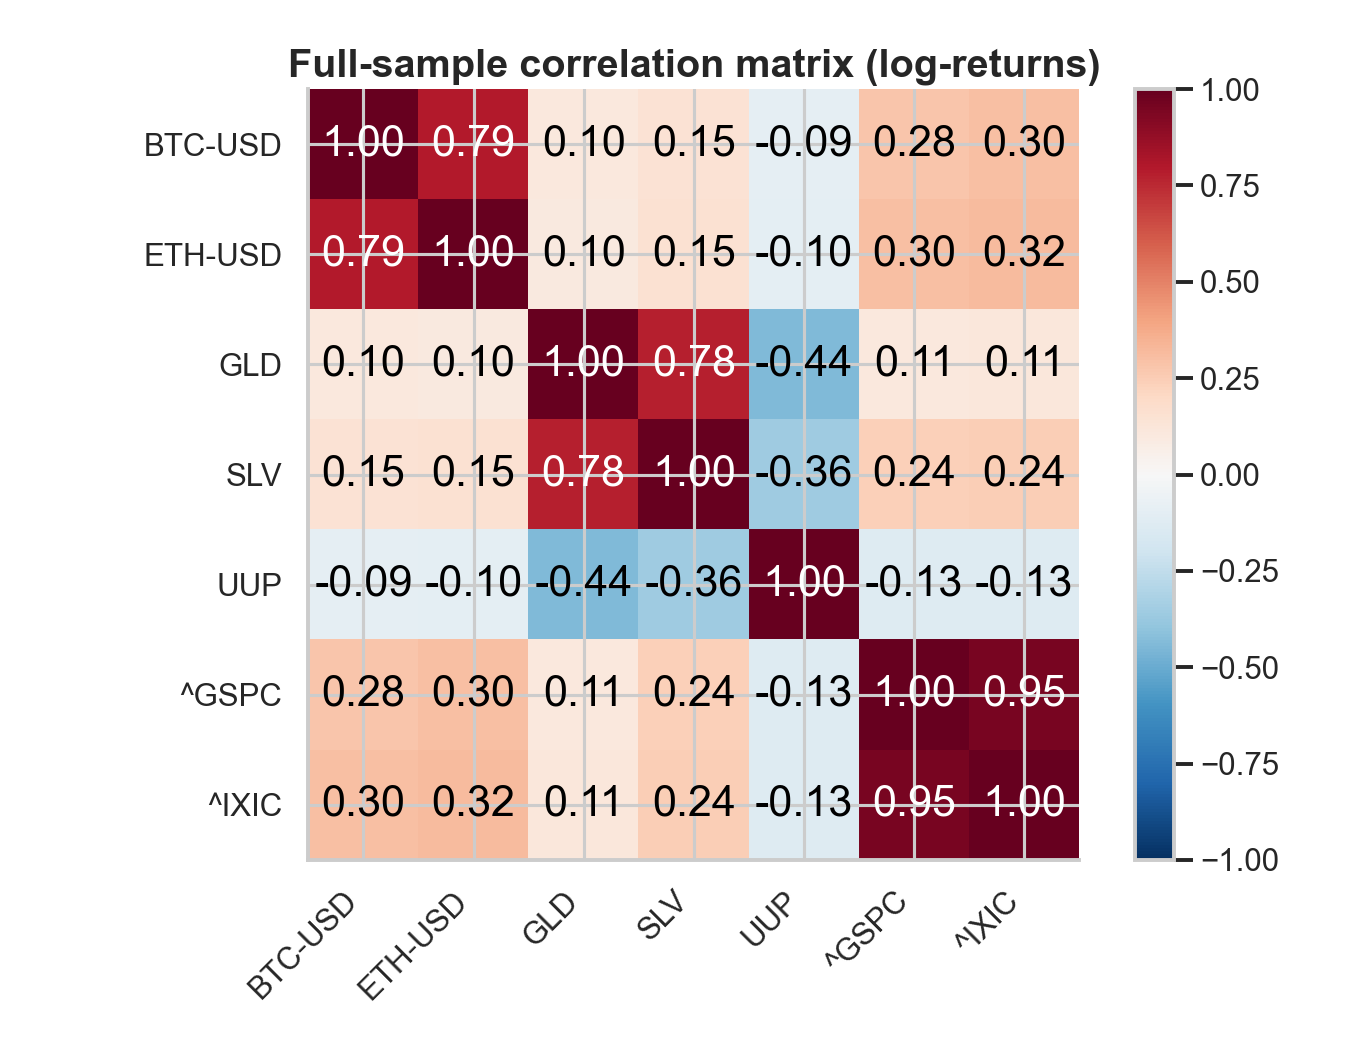
\includegraphics[width=0.85\textwidth]{../outputs/figures/eda_corr_heatmap.png}
    \caption{Static correlation heatmap of the return series.}
    \label{fig:eda_heatmap_appendix}
\end{figure}

\subsection{Dataset validation and quality diagnostics}

All price series are checked systematically before any modelling step. The diagnostics cover four areas: observation coverage, missing-value frequency, extreme-return events, and distributional shape. Table~\ref{tab:data_quality} summarises the results for each ticker.

\begin{table}[H]
\centering
\small
\caption{Data quality summary per ticker}
\label{tab:data_quality}
\resizebox{\textwidth}{!}{%
\begin{tabular}{lrrrrrrrrr}
\toprule
Ticker & First obs. & Last obs. & N & \% miss. & Gaps $>$2d & Zero ret. & Skew & Ex.Kurt & Ann.Vol (\%) \\
\midrule
BTC-USD & 2017-11-09 & 2026-05-16 & 3053 & 0.00 & 0 & 0 & -0.73 & 13.48 & 55.88 \\
ETH-USD & 2017-11-09 & 2026-05-16 & 3053 & 0.00 & 0 & 0 & -0.74 & 10.86 & 72.40 \\
GLD & 2017-11-09 & 2026-05-16 & 3053 & 0.00 & 0 & 920 & -0.87 & 13.63 & 13.88 \\
SLV & 2017-11-09 & 2026-05-16 & 3053 & 0.00 & 0 & 955 & -2.69 & 49.30 & 28.49 \\
UUP & 2017-11-09 & 2026-05-16 & 3053 & 0.00 & 0 & 1001 & -0.03 & 8.56 & 5.84 \\
\^{}GSPC & 2017-11-09 & 2026-05-16 & 3053 & 0.00 & 0 & 914 & -0.74 & 22.67 & 16.15 \\
\^{}IXIC & 2017-11-09 & 2026-05-16 & 3053 & 0.00 & 0 & 915 & -0.46 & 12.66 & 19.62 \\
\bottomrule
\end{tabular}
}
\end{table}

Figure~\ref{fig:dq_coverage} confirms that all seven tickers share an uninterrupted observation window from November 2017 to May 2026, with no gaps in coverage after alignment.

\begin{figure}[H]
    \centering
    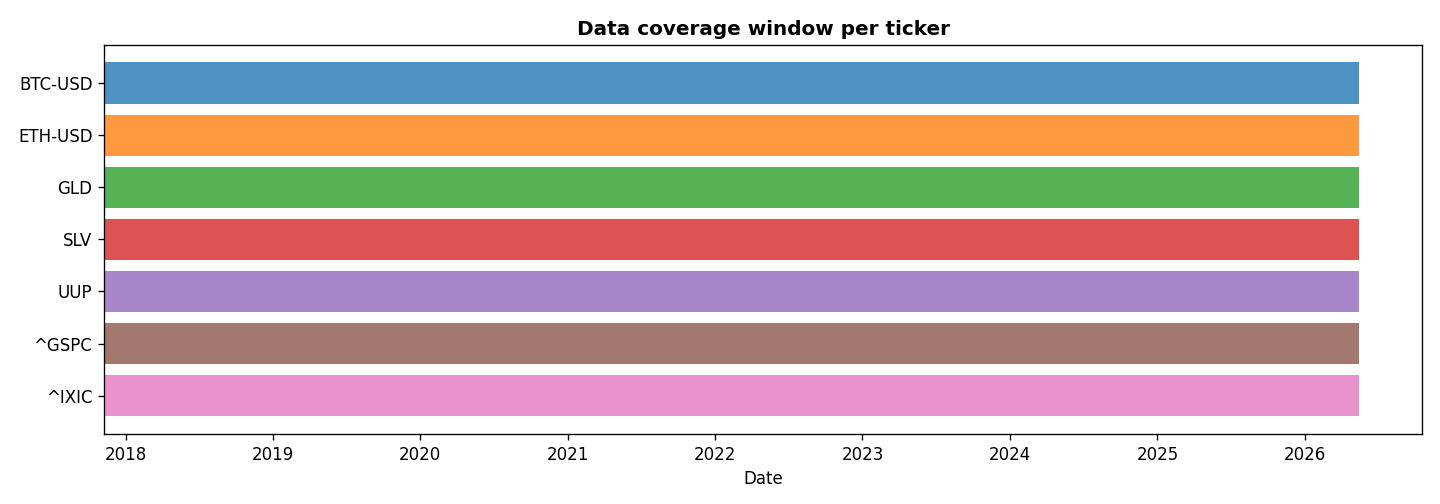
\includegraphics[width=0.88\textwidth]{../outputs/figures/fig_price_coverage.png}
    \caption{Observation coverage window per ticker. All assets share the aligned date range after the ETH-USD availability cutoff in November 2017.}
    \label{fig:dq_coverage}
\end{figure}

Figure~\ref{fig:dq_outliers} shows extreme return events ($|z\text{-score}| > 5\sigma$) for each asset. Bitcoin and Ethereum contain the outliers with the largest absolute magnitude. This is consistent with the well-known fat-tailed behaviour of crypto returns, with excess kurtosis of 13.5 for Bitcoin. However, Bitcoin and Ethereum are not the most leptokurtic series in the sample. Silver has an excess kurtosis of 49.3, while the S\&P~500 has 22.7.

These values are not directly comparable with the crypto series because the moments for the five conventional assets are calculated from return vectors in which about 30\% of the observations are forced to zero for weekends. This reduces the variance and increases the standardised fourth moment. All five conventional assets therefore contain a large number of zero-return days. This is not an ETF-specific issue. It results from aligning five-day-a-week assets with Bitcoin's seven-day trading calendar. Weekend gaps are filled with zeros, so every Saturday and Sunday receives a forced zero return, while the continuously traded crypto assets do not contain such observations.

This calendar difference is a genuine limitation. On weekend days, a real Bitcoin return is paired with a zero conventional-asset return, which mechanically reduces the rolling correlation. A further concern is that forward-filling could make the target more persistent. This matters because persistence is an important part of the results in Chapters~\ref{sec:results_overview} and~\ref{sec:discussion}.

To examine this directly, the 30-day Bitcoin--S\&P~500 rolling correlation was recalculated using common trading days only. The 914 weekend and holiday rows were removed, and the persistence of this version was compared with the full-calendar version. The persistence is essentially unchanged and is even slightly higher without the weekend rows. The lag-1 autocorrelation of the Fisher-$z$ target is 0.977 with the seven-day calendar and 0.981 with trading days only. The naive ``tomorrow-equals-today'' $R^2$ is 0.954 compared with 0.961. The same pattern is observed for the 14-day and 90-day windows.

The forced weekend zeros therefore add some noise rather than creating artificial persistence. The dominant role of persistence is not a consequence of the calendar convention. Restricting the analysis to common trading days would be a useful refinement for future work, but it would not change the main findings. None of the detected outliers are data errors. They represent genuine price events and are therefore retained in the analysis.

\begin{figure}[H]
    \centering
    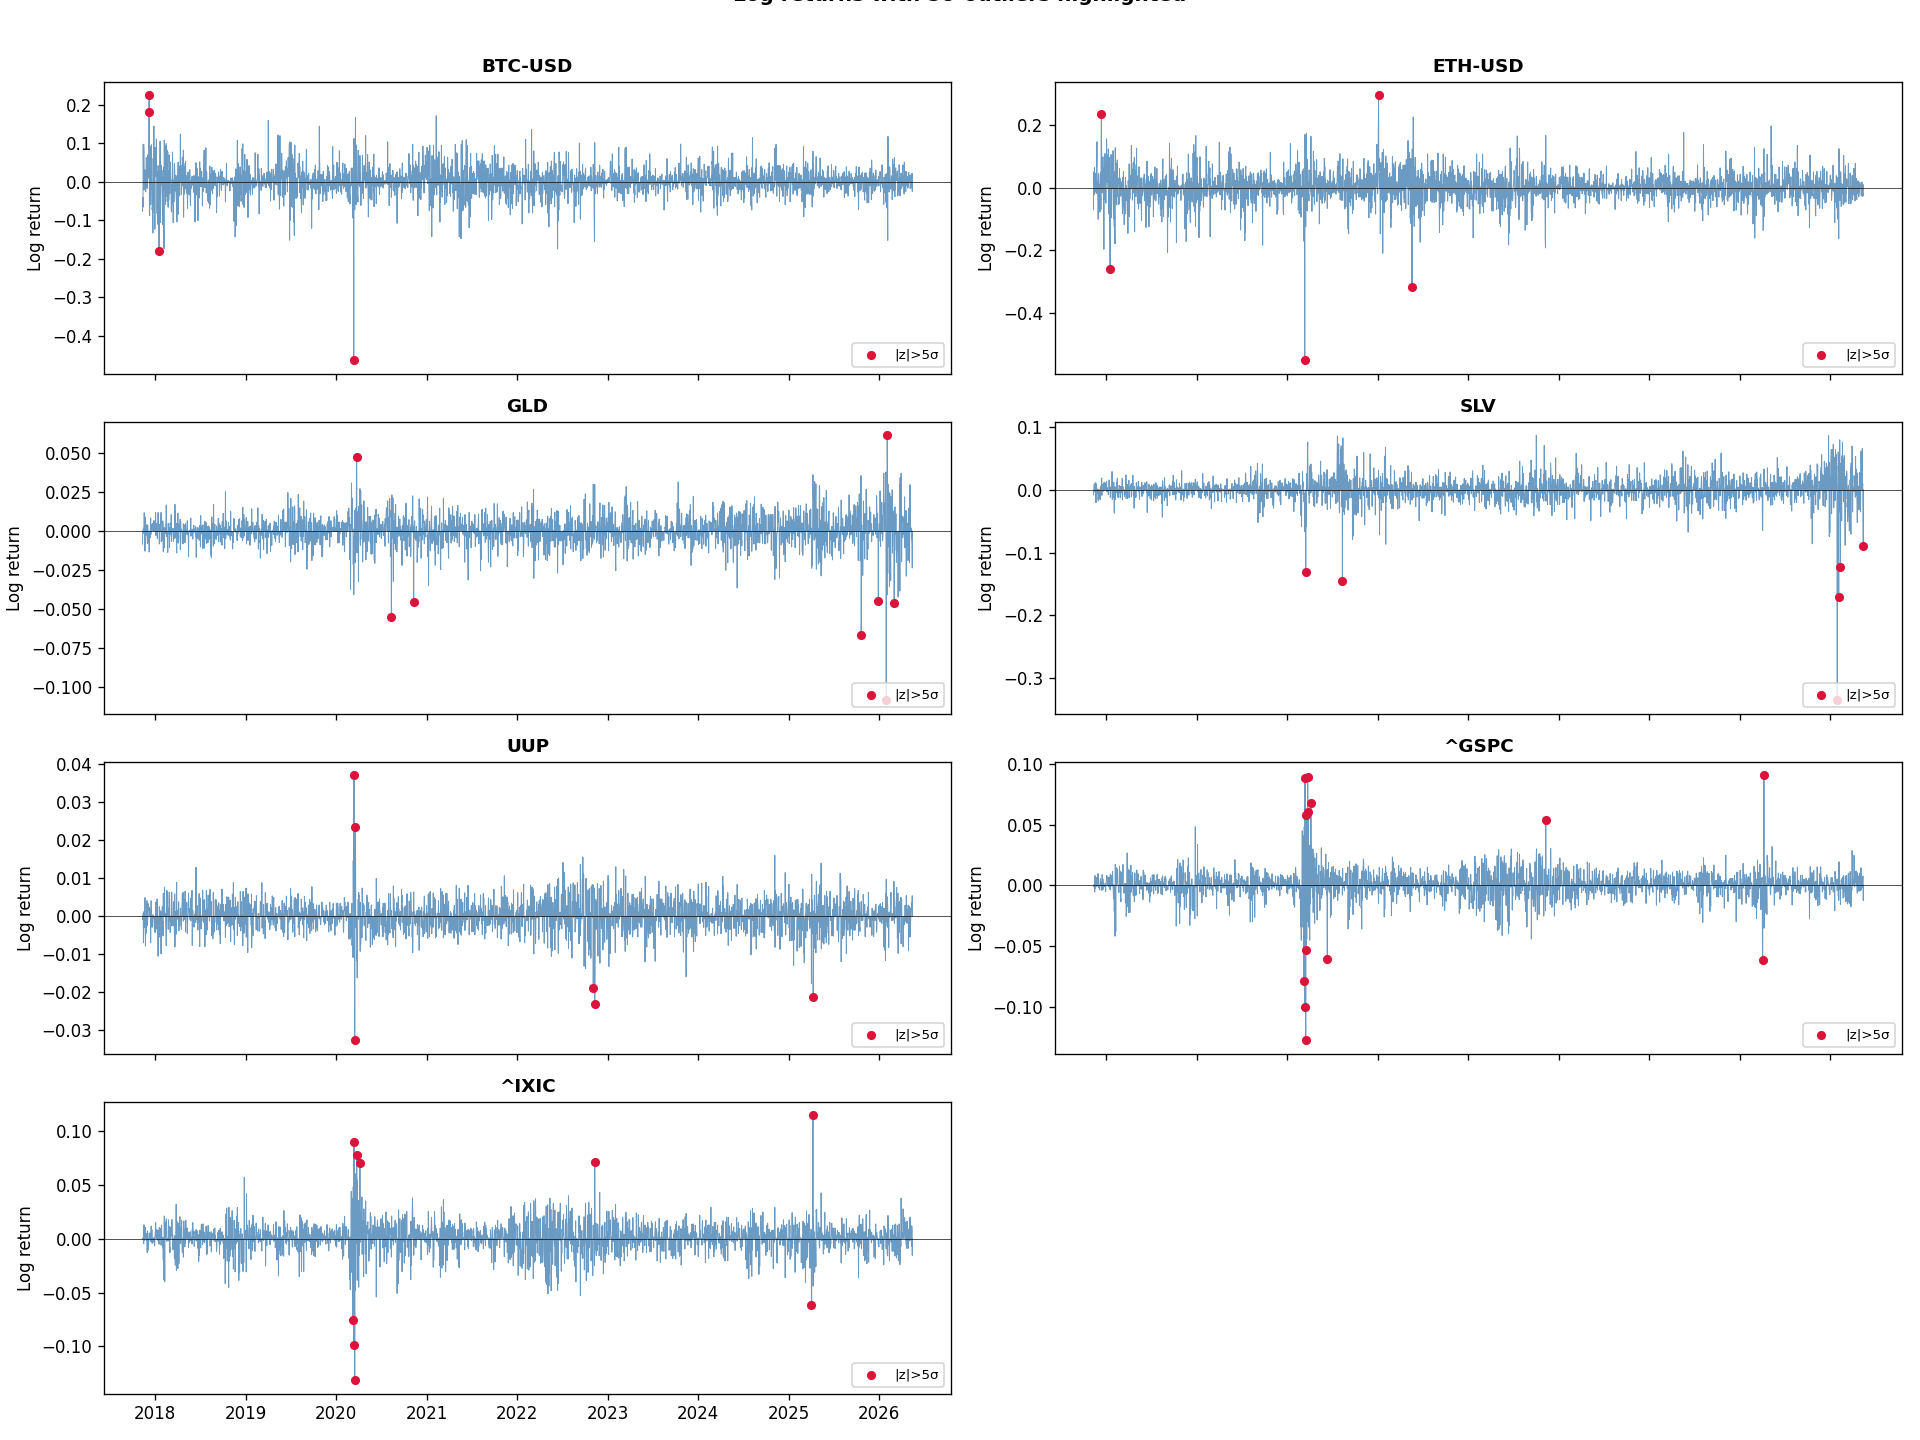
\includegraphics[width=0.95\textwidth]{../outputs/figures/fig_return_outliers.png}
    \caption{Log-return series with extreme observations ($|z| > 5\sigma$) highlighted in red. Crypto assets contain occasional large outliers, while conventional assets are more contained but are not free of extreme observations.}
    \label{fig:dq_outliers}
\end{figure}

\subsection{Fisher-z transformation of the correlation target}

The rolling Pearson correlation $\rho_t$ is bounded between $-1$ and $1$ and has compressed variance near the boundaries. Applying the Fisher-z transformation $z_t = \tanh^{-1}(\rho_t)$ maps the target onto the real line and makes the variance more stable across the range of correlations.

Figure~\ref{fig:eda_fisher} illustrates the distributional improvement for the representative Bitcoin--S\&P~500 pair at the 30-day window. The untransformed correlation distribution is left-skewed and bounded, while the Fisher-transformed version is more symmetric and approximately Gaussian.

\begin{figure}[H]
    \centering
    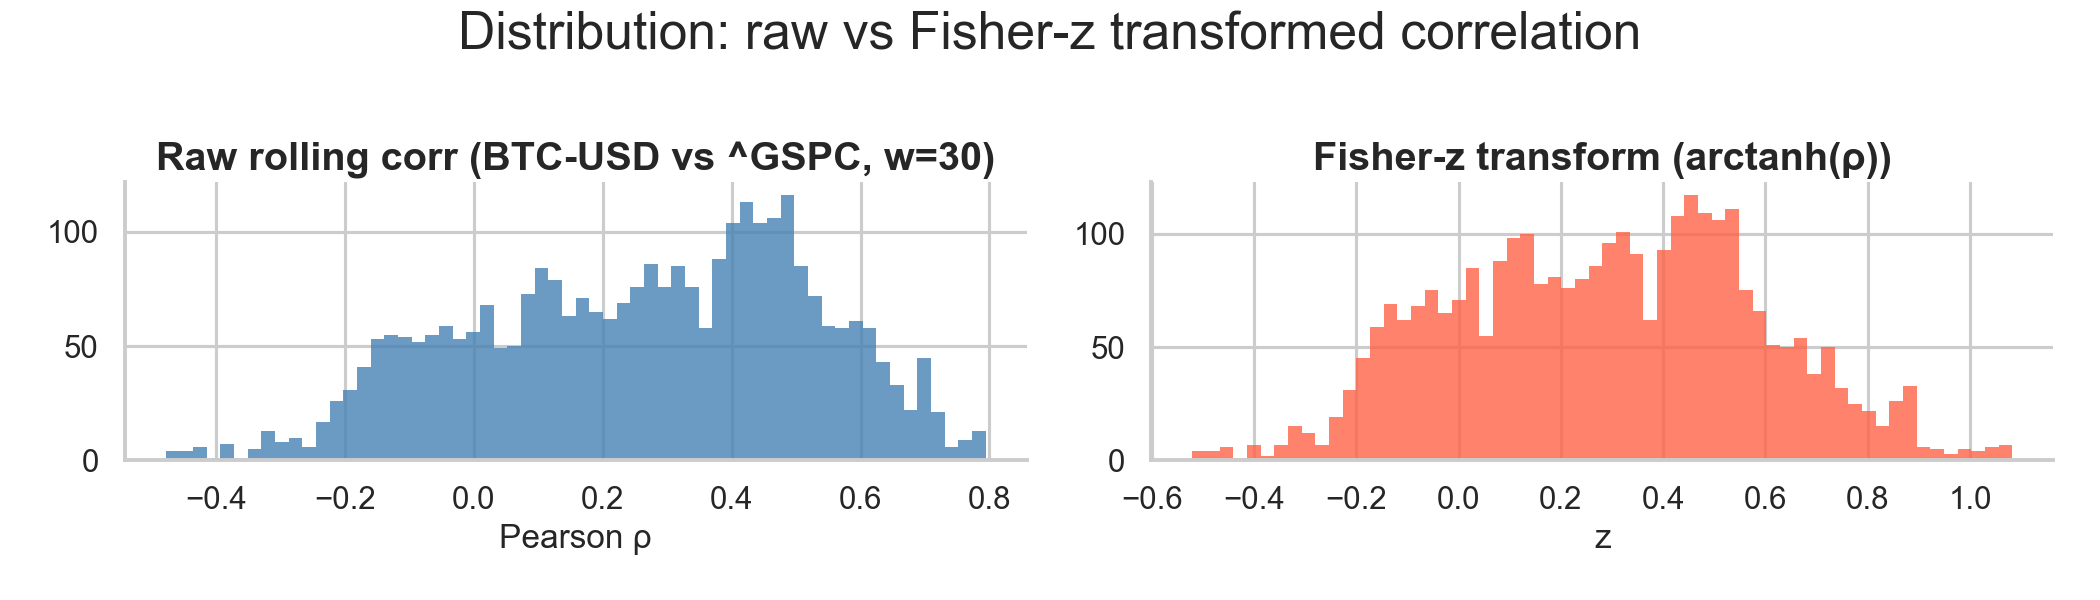
\includegraphics[width=0.88\textwidth]{../outputs/figures/eda_fisher_transform.png}
    \caption{Distribution of the 30-day rolling correlation before and after Fisher-z transformation for the Bitcoin--S\&P~500 pair. The transformation improves normality and reduces boundary compression.}
    \label{fig:eda_fisher}
\end{figure}

\subsection{Why multiple rolling windows are used}

The thesis uses 14-, 30-, 60-, and 90-day windows because no single time horizon is appropriate for every purpose. A short window reacts quickly to recent shocks but is noisier. A long window is smoother and more persistent but slower to capture a change in the underlying regime. Using all four windows makes it possible to examine these differences.

The choice of window length also shapes the overall forecastability profile. Longer windows are easier to forecast because they are smoother, but this forecasting success is largely explained by persistence. Shorter windows are noisier, but they can provide more information about local instability.

\subsection{Additional implementation remarks}

Each time the pipeline is run, the agreed results are written to the \texttt{outputs/results}, \texttt{outputs/tables}, \texttt{outputs/figures}, and \texttt{outputs/predictions} folders. This supports reproducibility and also makes the reporting process easier. Since the tables and figures are generated directly from the code, the gap between running the experiment and preparing the report is kept small.

The notebooks were developed in line with the main development process and were not allowed to drift away from it. The figures produced in the notebooks remain interpretable, the control metrics are selected consistently, and helper functions are reused without relying on fragile path assumptions.

This is important in practice because research notebooks can easily diverge from the code used to produce the results and become unreliable over time.

\subsection{Summary}

The conclusion is mainly methodological: the environment studied here is heterogeneous, economically non-stationary, and sufficiently complex to justify treating the relationship as time-varying. The descriptive evidence supports the modelling strategy presented in the main text.
